% Yahboom ROSMASTER X3: dimensions used by the simulator (schematic, own drawing).
% Values from the manufacturer's published dimensions, see docs/paper_reference.md section 8.
% Build:  pdflatex rosmaster_x3_dimensions.tex
%         pdftoppm -png -r 200 -singlefile rosmaster_x3_dimensions.pdf rosmaster_x3_dimensions
% Coordinates are in millimetres (x = 0.3 mm on paper per mm of robot), origin = robot center.
\documentclass[tikz,border=4mm]{standalone}
\usepackage{amsmath,amssymb}
\usetikzlibrary{arrows.meta}

\tikzset{
  body/.style   = {draw, thick, fill=gray!12},
  wheel/.style  = {draw, thick, fill=gray!55},
  dim/.style    = {{Latex[length=2mm]}-{Latex[length=2mm]}, thin},
  ext/.style    = {thin, gray},
  axis/.style   = {-{Latex[length=2.5mm]}, very thick},
  lbl/.style    = {font=\small, fill=white, inner sep=1pt},
}

\begin{document}
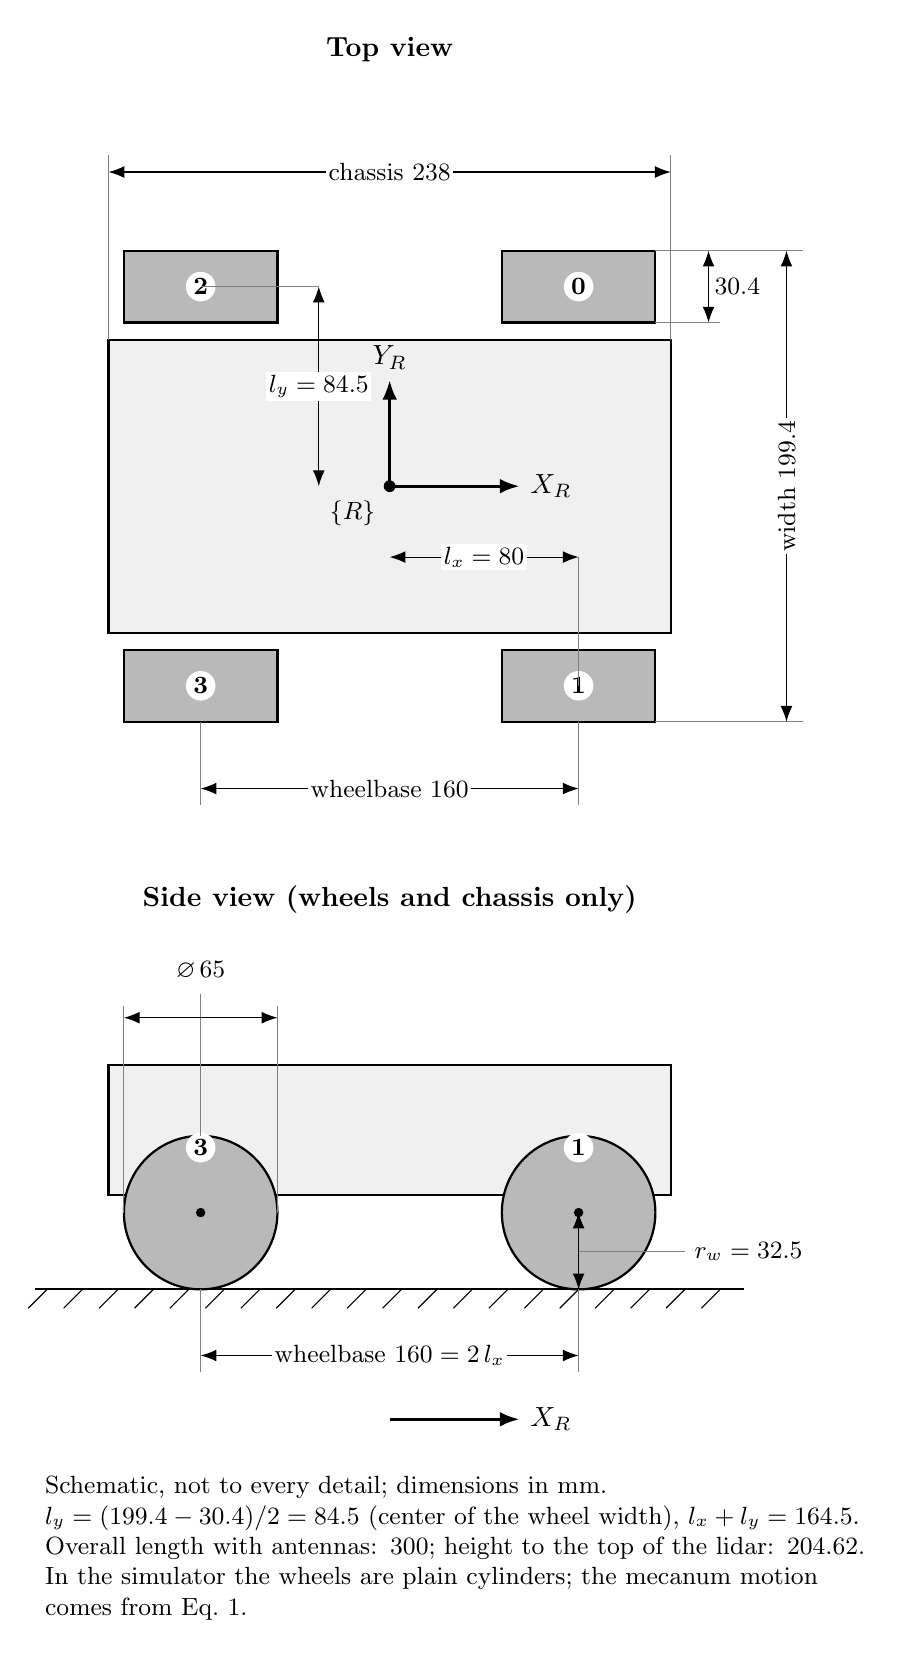
\begin{tikzpicture}[x=0.3mm, y=0.3mm]

% =====================================================================
% TOP VIEW (X_R forward = to the right, Y_R left = up)
% =====================================================================
\node[font=\bfseries] at (0,185) {Top view};

% chassis: 238 mm long, between the inner faces of the wheels
\draw[body] (-119,-62) rectangle (119,62);

% wheels: 65 mm long (diameter), 30.4 mm wide, centers at (+-l_x, +-l_y)
% numbering of Fig. 6 of the paper: 0 front-left, 1 front-right, 2 rear-left, 3 rear-right
\foreach \x/\y/\n in {80/84.5/0, 80/-84.5/1, -80/84.5/2, -80/-84.5/3} {
  \draw[wheel] (\x-32.5,\y-15.2) rectangle (\x+32.5,\y+15.2);
  \node[font=\small\bfseries, fill=white, circle, inner sep=1pt] at (\x,\y) {\n};
}

% robot frame {R} at the center
\fill (0,0) circle (2.5);
\draw[axis] (0,0) -- (55,0)  node[right] {$X_R$};
\draw[axis] (0,0) -- (0,45)  node[above] {$Y_R$};
\node[font=\small, anchor=north east] at (-2,-2) {$\{R\}$};

% l_x and l_y (the parameters of Eq. 1)
\draw[ext] (80,-84.5) -- (80,-30);
\draw[dim] (0,-30) -- node[lbl] {$l_x = 80$} (80,-30);
\draw[ext] (-80,84.5) -- (-30,84.5);
\draw[dim] (-30,0) -- node[lbl] {$l_y = 84.5$} (-30,84.5);

% wheelbase 160 mm (below the robot)
\draw[ext] (80,-100) -- (80,-135);
\draw[ext] (-80,-100) -- (-80,-135);
\draw[dim] (-80,-128) -- node[lbl] {wheelbase 160} (80,-128);

% chassis length 238 mm (above the robot)
\draw[ext] (-119,62) -- (-119,140);
\draw[ext] (119,62) -- (119,140);
\draw[dim] (-119,133) -- node[lbl] {chassis 238} (119,133);

% overall width 199.4 mm (outer wheel faces) and wheel width 30.4 mm (right side)
\draw[ext] (112.5,99.7) -- (175,99.7);
\draw[ext] (112.5,-99.7) -- (175,-99.7);
\draw[dim] (168,-99.7) -- node[lbl, rotate=90] {width 199.4} (168,99.7);
\draw[ext] (112.5,69.3) -- (140,69.3);
\draw[dim] (135,69.3) -- node[lbl, right=1pt, fill=none] {30.4} (135,99.7);

% =====================================================================
% SIDE VIEW (seen from the right side, X_R forward = to the right)
% =====================================================================
\begin{scope}[yshift=-102mm]   % = -340 drawing units (0.3 mm each)
  \node[font=\bfseries] at (0,165) {Side view (wheels and chassis only)};

  % ground
  \draw[thick] (-150,0) -- (150,0);
  \foreach \x in {-145,-130,...,145} \draw[thin] (\x,0) -- (\x-8,-8);

  % chassis (schematic block) and the two wheels on this side
  \draw[body] (-119,40) rectangle (119,95);
  \draw[wheel] (80,32.5) circle (32.5);
  \draw[wheel] (-80,32.5) circle (32.5);
  \fill (80,32.5) circle (2);  \fill (-80,32.5) circle (2);
  \node[font=\small\bfseries, fill=white, circle, inner sep=1pt] at (80,60) {1};
  \node[font=\small\bfseries, fill=white, circle, inner sep=1pt] at (-80,60) {3};

  % wheel diameter 65 mm and radius r_w
  \draw[dim] (80,0) -- (80,32.5);
  \draw[ext] (80,16) -- (125,16) node[right, font=\small, black] {$r_w = 32.5$};
  \draw[ext] (-80,65) -- (-80,125);
  \node[font=\small] at (-80,135) {$\varnothing\,65$};
  \draw[dim] (-112.5,115) -- (-47.5,115);
  \draw[ext] (-112.5,32.5) -- (-112.5,120);
  \draw[ext] (-47.5,32.5) -- (-47.5,120);

  % wheelbase 160 mm between the axles
  \draw[ext] (80,0) -- (80,-35);
  \draw[ext] (-80,0) -- (-80,-35);
  \draw[dim] (-80,-28) -- node[lbl] {wheelbase $160 = 2\,l_x$} (80,-28);

  \draw[axis] (0,-55) -- (55,-55) node[right] {$X_R$};
\end{scope}

% =====================================================================
% Notes
% =====================================================================
\node[align=left, font=\small, anchor=north west, text width=105mm] at (-150,-415) {%
  Schematic, not to every detail; dimensions in mm.\\
  $l_y = (199.4 - 30.4)/2 = 84.5$ (center of the wheel width), $l_x + l_y = 164.5$.\\
  Overall length with antennas: 300; height to the top of the lidar: 204.62.\\
  In the simulator the wheels are plain cylinders; the mecanum motion comes from Eq.~1.};

\end{tikzpicture}
\end{document}
